\documentclass[10pt,a4paper,oneside]{beamer}

\usetheme{Boadilla}

\usepackage[utf8]{inputenc}
\usepackage[german]{babel}
\usepackage{amsmath}
\usepackage{amsfonts}
\usepackage{amssymb}
\usepackage{hyperref}
\usepackage{biblatex}
\usepackage{wrapfig}
\addbibresource{bib}
\usepackage{verbatim}
\usepackage{subfigure}

\title{Inertialnavigation von autonomen Flugkörpern}
\author{
	Fabian Ulbricht \and
	Paul Walger 
}

\begin{document}

%% Start
\frame{
	\titlepage
}

\frame {
	\frametitle{Gliederung}
	\tableofcontents
}

\begin{frame}
  \section{Einleitung}
  \frametitle{Einleitung}
  \begin{definition}[Inertialnavigation]
  Feststellung von Position, Richtung und Geschwindigkeit\\
  und Navigation nur mit Hilfe von
  \begin{itemize}
  \item Beschleunigungssensoren
  \item Drehratensensoren
  \end{itemize}
  und der damit verbundenen Messung der 6 Freiheiten ohne andere Daten von Außen
  \end{definition}
  Anwendung:
  \begin{figure}[htbp]
      \begin{minipage}{0.3\textwidth}
       \centering
        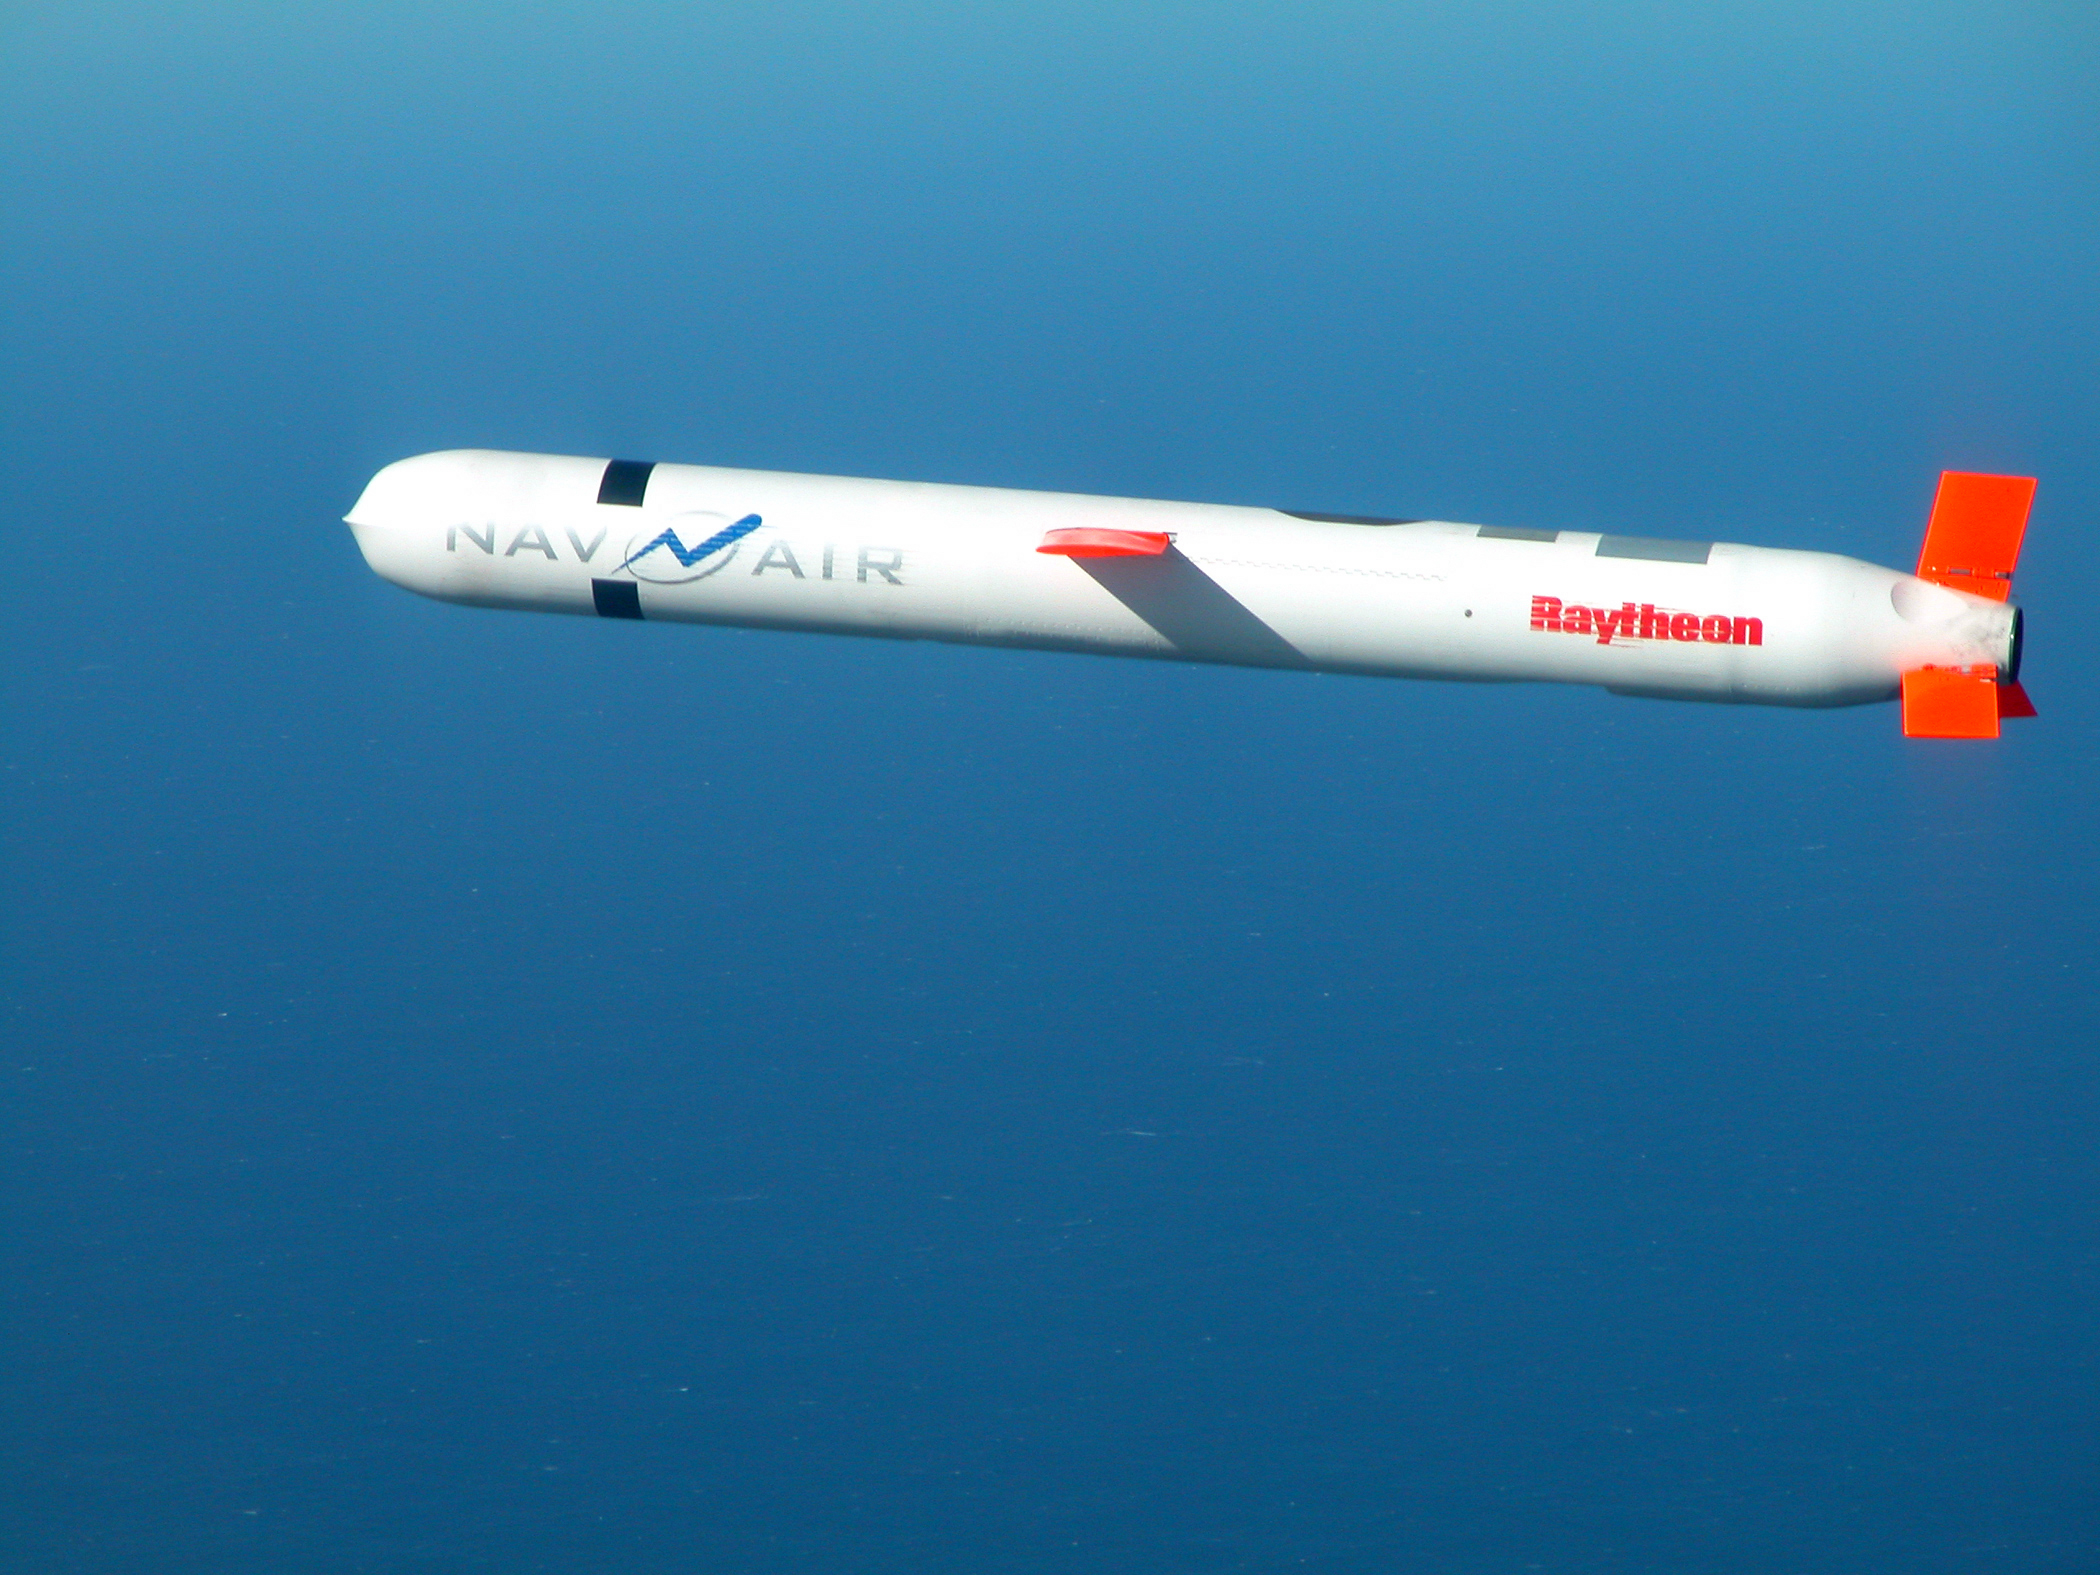
\includegraphics[width=0.8\textwidth]{images/cruise_missle.jpg}
        \caption{Bild links}
      \end{minipage}\hfill
      \begin{minipage}{0.3\textwidth}
       \centering
        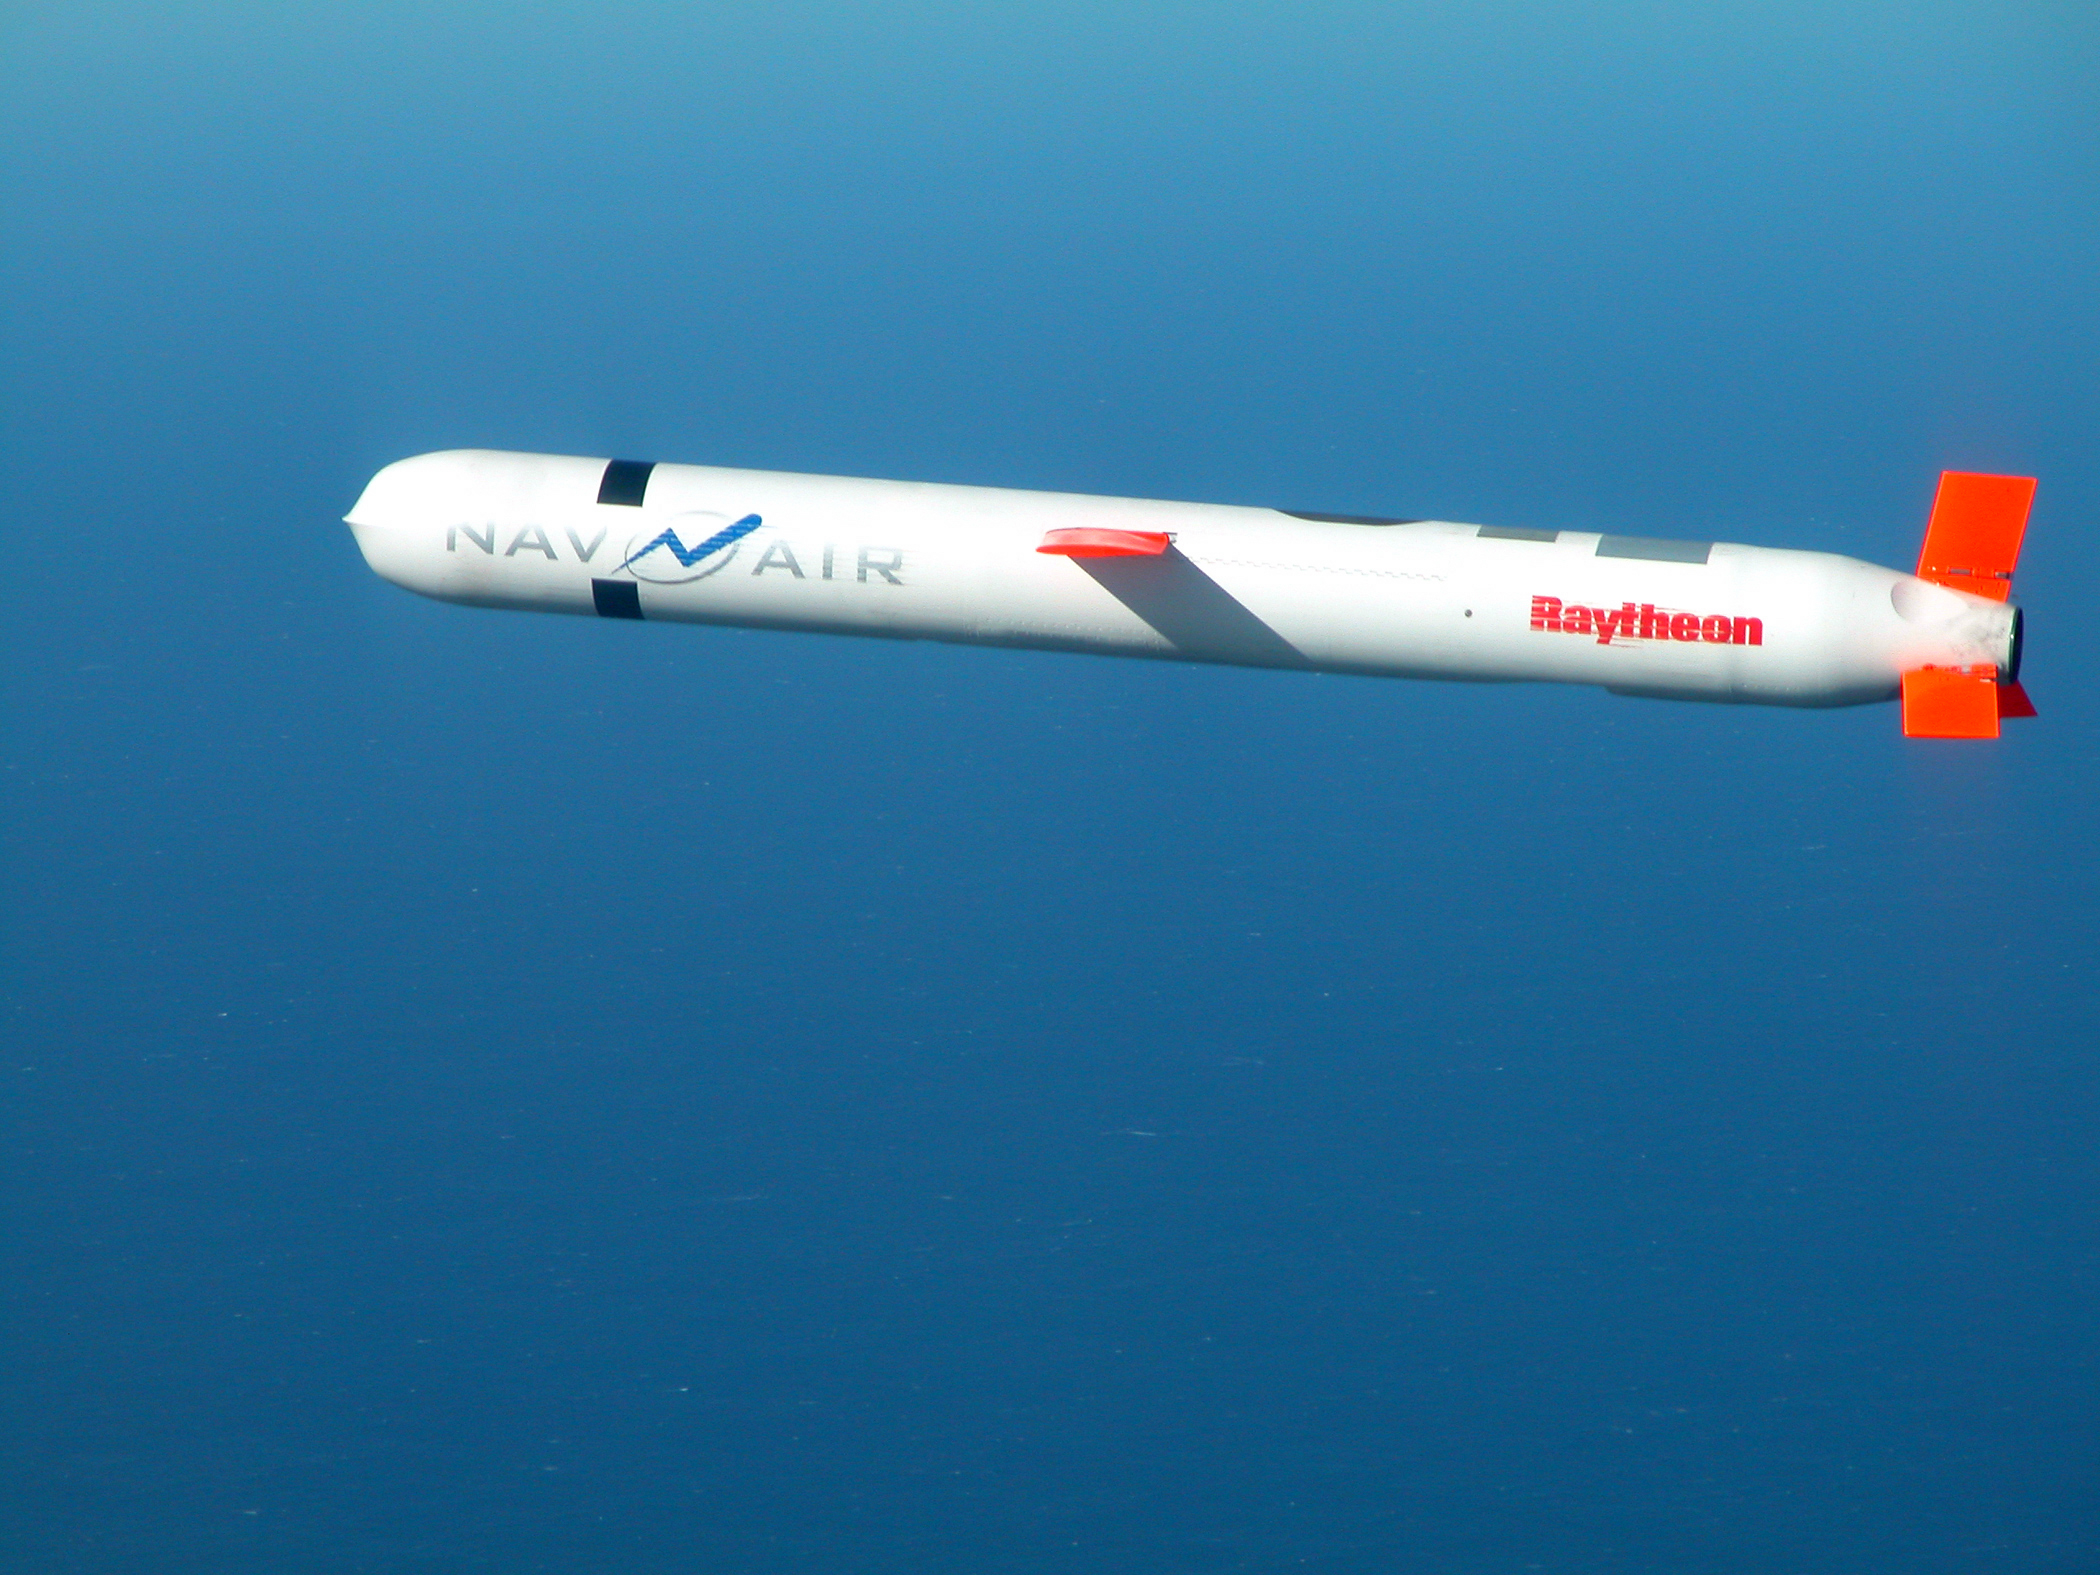
\includegraphics[width=0.8\textwidth]{images/cruise_missle.jpg}
        \caption{Bild rechts}
      \end{minipage}\hfill
      \begin{minipage}{0.3\textwidth}
       \centering
        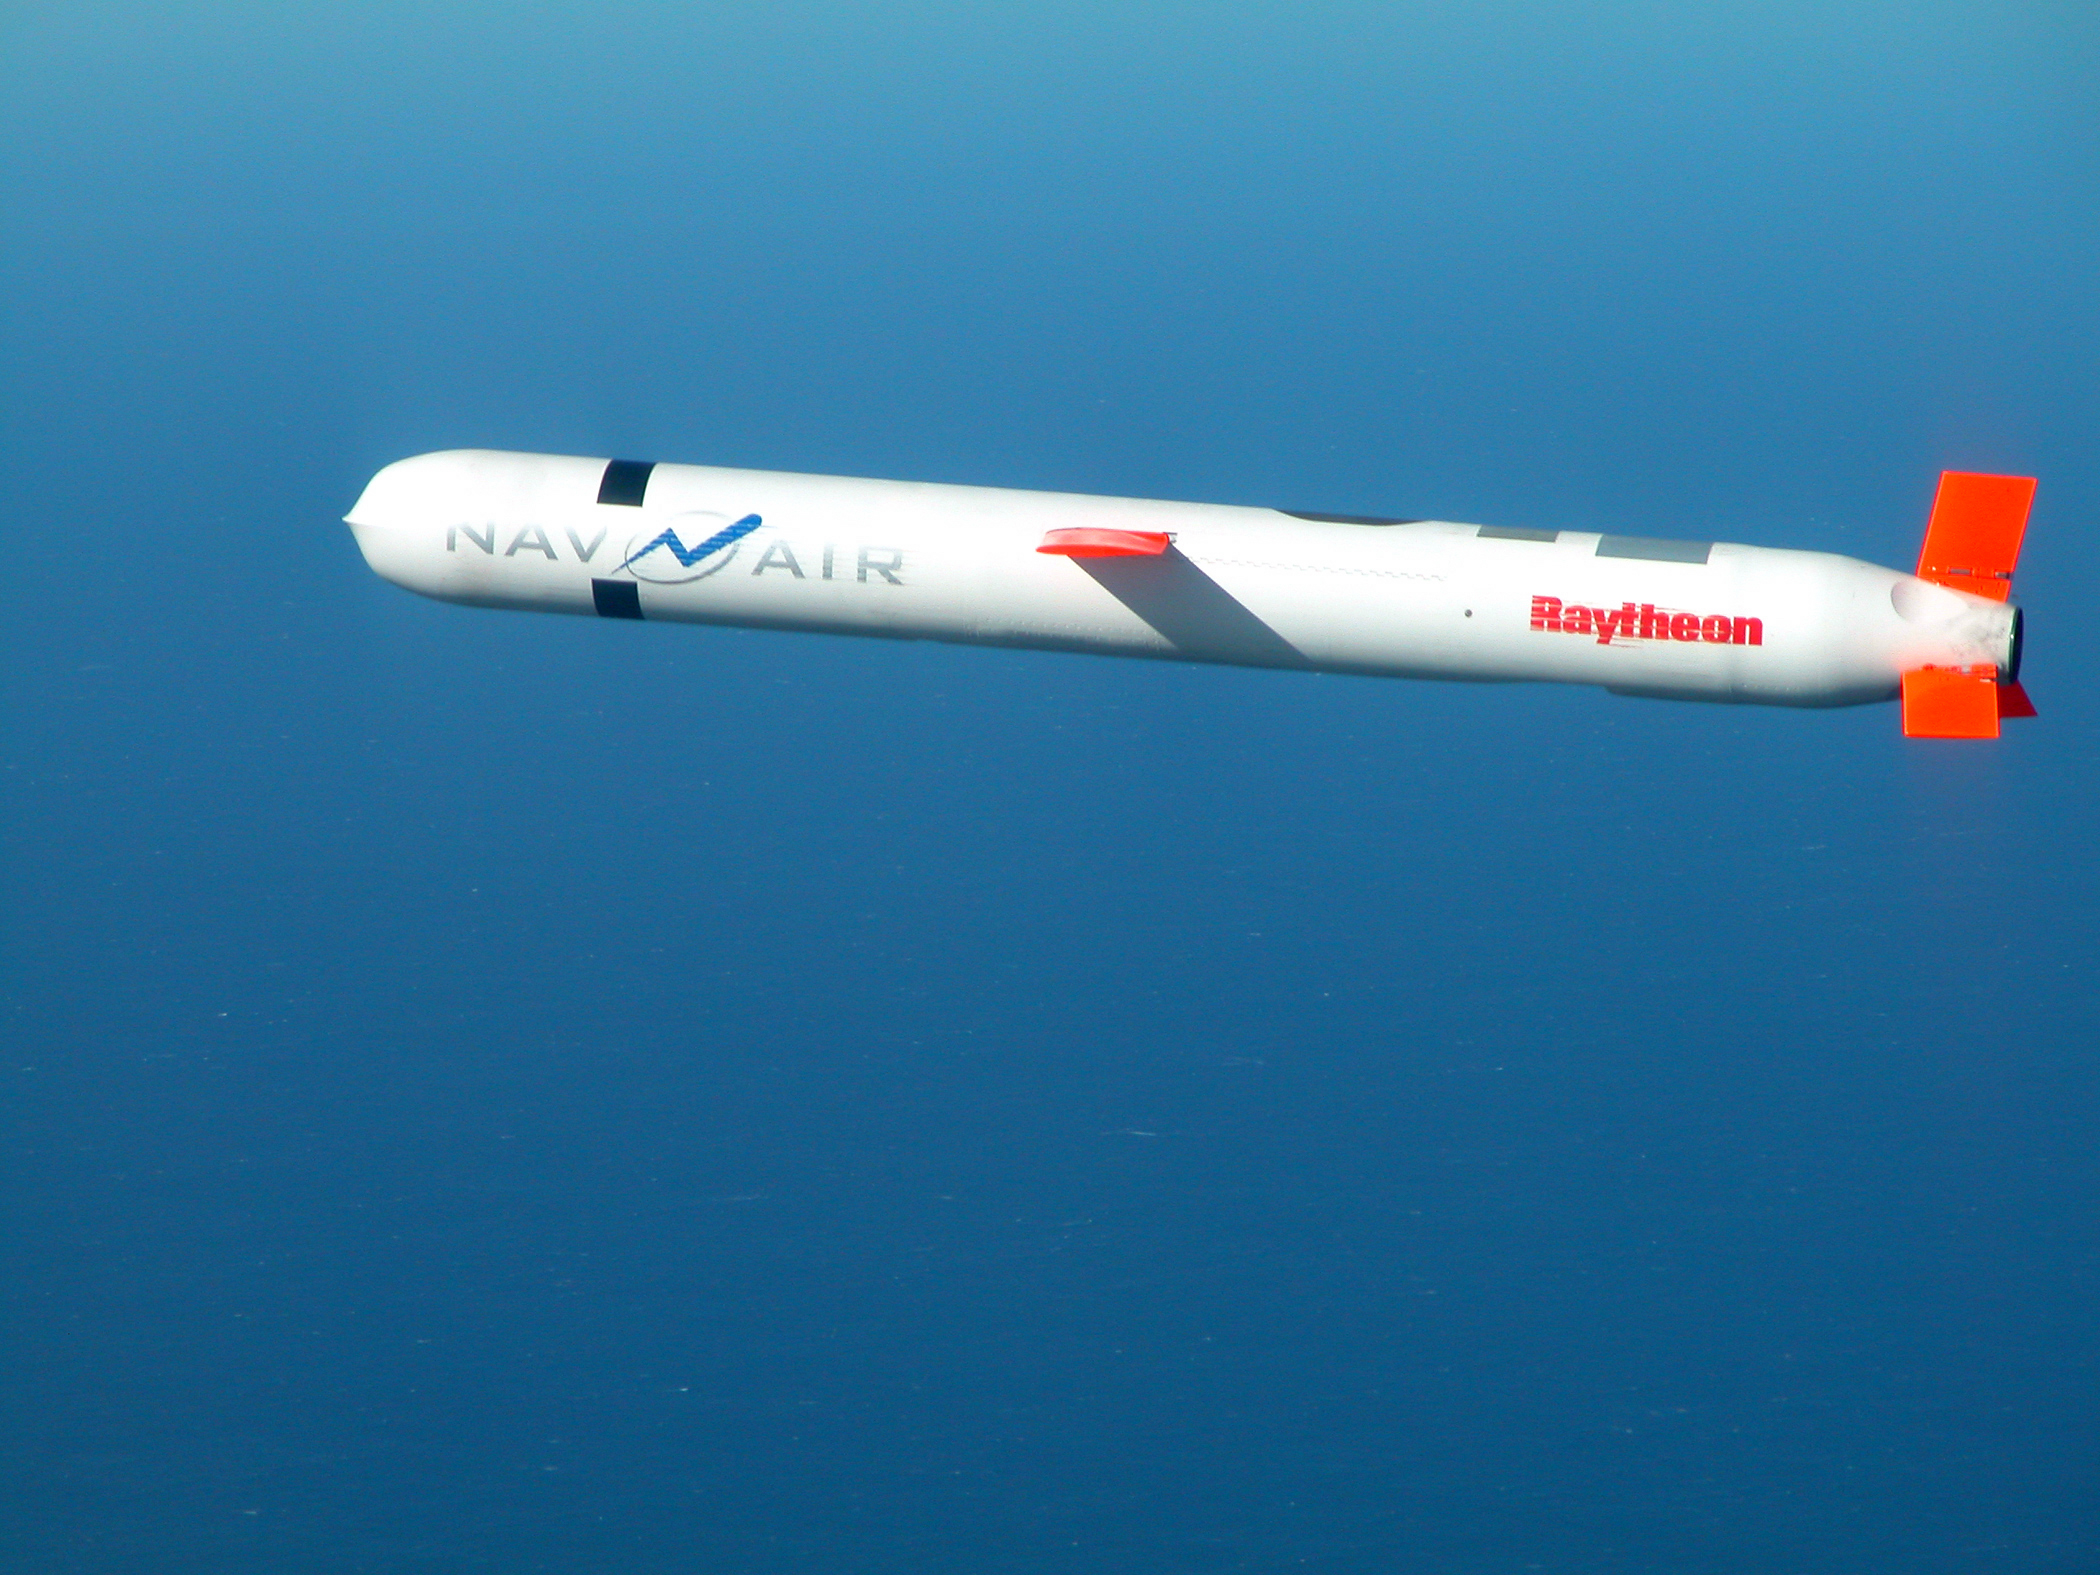
\includegraphics[width=0.8\textwidth]{images/cruise_missle.jpg}
        \caption{Bild rechts}
      \end{minipage}
    \end{figure}
\end{frame}

\begin{frame}
	\subsection{Acceleromter}
	\frametitle{Accelerometer (Beschleunigungssensoren)}
	\begin{block}{Prinzip}
		Messung der aufgrund von Trägheitskräften resultierende Beschleunigung
	\end{block}
	Anwendung:
	\begin{itemize}
    	\item Messung von (linearen) Beschleunigungen
  		\item Sensorik in digitalen Kameras
		\item Positionsbestimmung
	\end{itemize}
	\begin{figure}
\subfigure{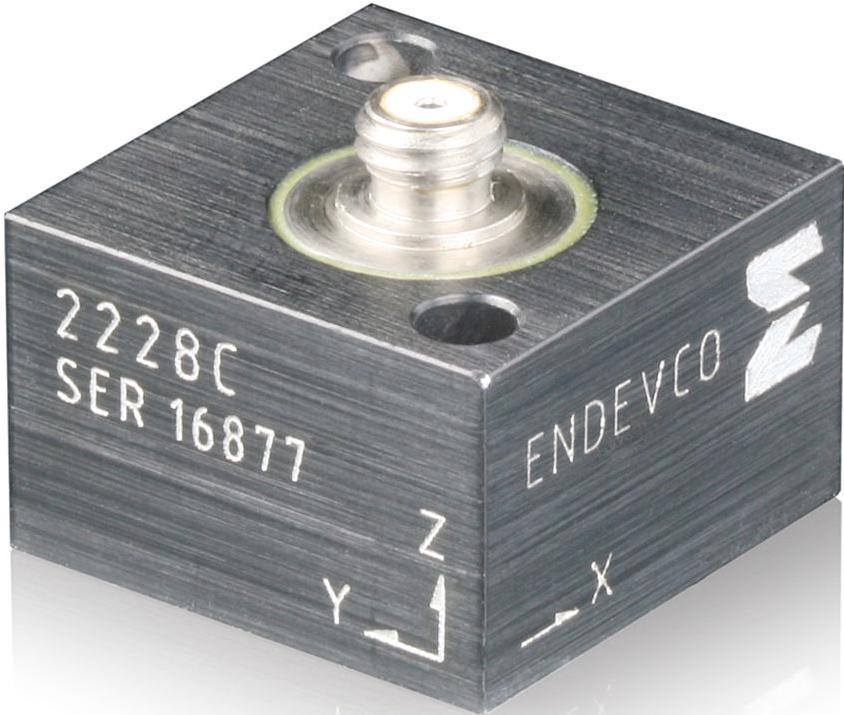
\includegraphics[width=0.49\textwidth, height=0.4\textheight,keepaspectratio=true]{images/acc2.jpg}}\hfil
\subfigure{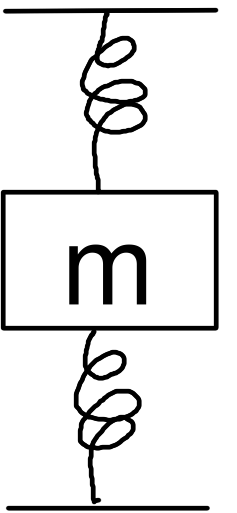
\includegraphics[width=0.49\textwidth, height=0.4\textheight,keepaspectratio=true]{images/acc.png}}\hfil
\end{figure}

\end{frame}

\begin{frame}
	\frametitle{Kapazitive Accelerometer}
	\begin{block}{Funktionsweise}
		Messung von Kapazitätsänderungen.
	\end{block}
 	\begin{definition}[MEMS]
  	= Microelectromechanical systems \\
  	Sehr kleine mechanische Geräte angetrieben durch Elektrizität.
  	\end{definition}
    \bigskip
   
	Vorteile
 	\begin{itemize}
 		\item Herstellung mit herkömmlicher MEMS Technologie möglich
 		\item Hervorragende Sensibilität
		\item Unabhängig von Außentemperatur
 	\end{itemize}
\end{frame}

\begin{frame}
	\frametitle{Kapazität}
	Die Kapazität von 2 parallen Platten ist \cite{AM08}
	\begin{equation}
		C_{0} = \epsilon_{0} \epsilon_{r} \frac{A}{d}
	\end{equation}
	\begin{itemize}
		\item $\epsilon_{0}$ = elektrische Feldkonstante
		\item $\epsilon_{r}$ = relative Permittivität
		\item $A$ = Fläche der Elektroden
		\item $d$ = Distanz zwischen den Elektroden
	\end{itemize}

\end{frame}

\begin{frame}
	\frametitle{Aufbau eines MEMS Accelerometer}
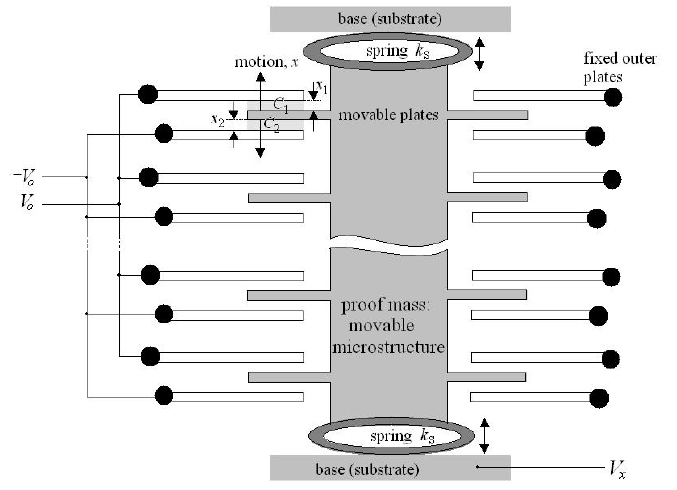
\includegraphics[width=\textwidth]{images/acceleromter_structure.png}

\end{frame}

\begin{frame}
  \subsection{Gyroskop}
  \frametitle{Gyroskop (Rotationssensoren)}
  
  \begin{block}{Was ist ein Gyroskop}
  	Ein Gerät zur Messung oder Erhaltung der Orientierung.
  \end{block}
  
  \bigskip
  
  Typen
  \begin{enumerate}
  	\item Mechanisch
  	\item Optisch
  	\item MEMS Gyroscope
  \end{enumerate}
  
	\begin{center}
  		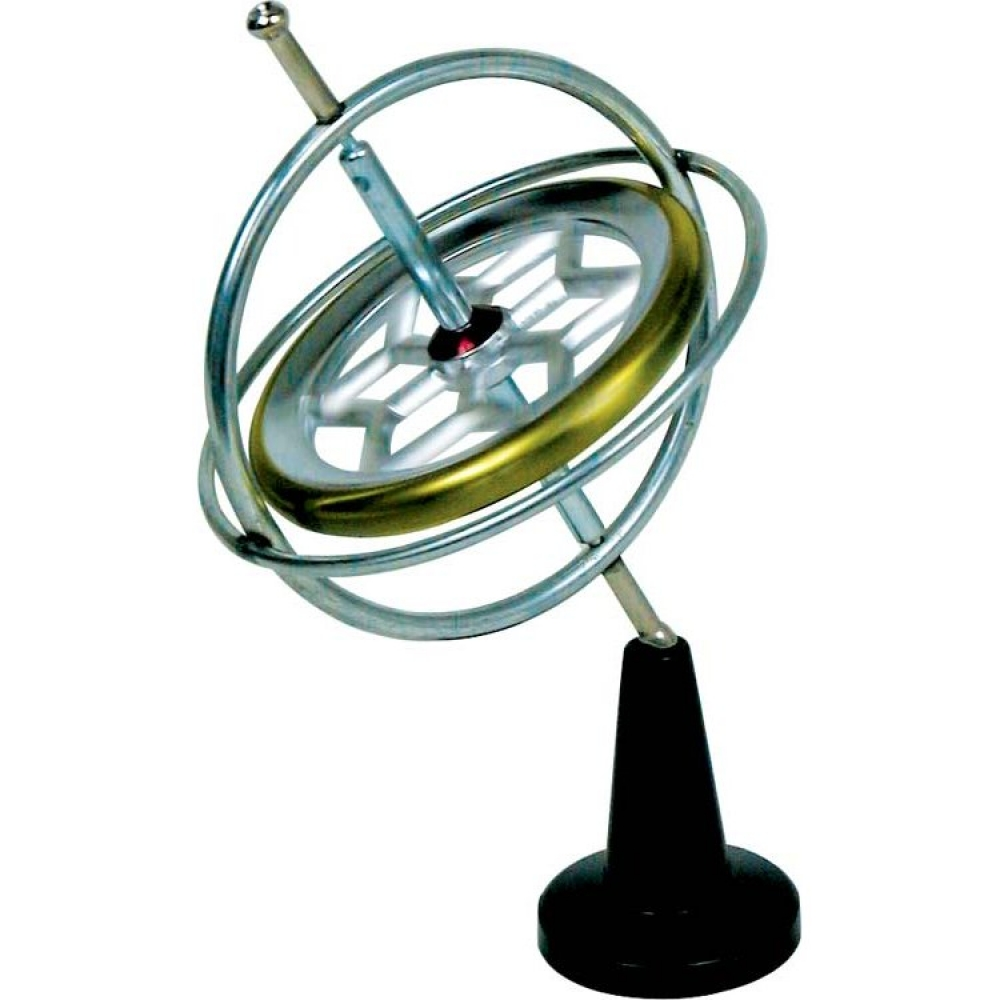
\includegraphics[scale=0.09]{images/Original_gyroscope-1000x1000.jpg} 
	\end{center}
\end{frame}

\begin{frame}
	\frametitle{Mechanische Gyroskope}
	%% http://www.ipgp.fr/~lucas/Contrib/animbeamer.html

	\begin{itemize}
		\item basiert aus dem Prinzip der Drehimpluserhaltung
		\item ein rotierendes Rad und zwei Kardanische Aufhängungen
		\item Nachteile:
		\begin{enumerate}
	  		\item Bewegliche Teile
	  		\item Reibung
	  		\item Ein paar Minuten Aufwärmzeit benötigt
	  	\end{enumerate}
	\end{itemize}

	\begin{center}
		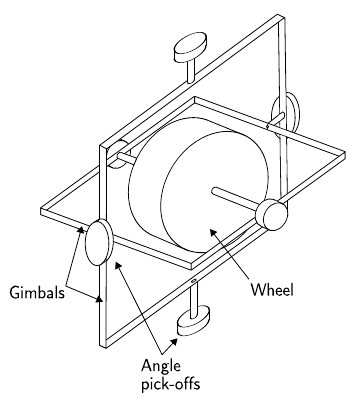
\includegraphics[width=0.35\textwidth]{images/mechanical_gyroscope.png} 
	\end{center}
\end{frame}

\begin{frame}
	\frametitle{Optische Gyroskope}
	\begin{wrapfigure}{l}{0.4\textwidth}
	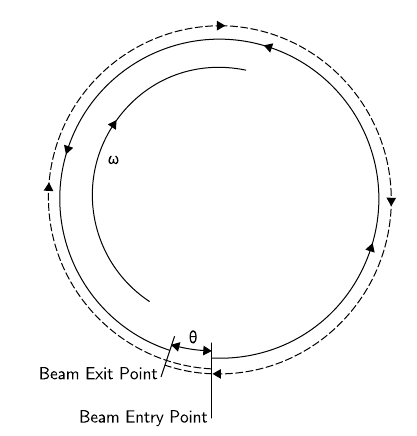
\includegraphics[width=0.4\textwidth]{images/fog.png} 
	\end{wrapfigure}
	
	Insbesondere Faserkreisel (Fibro Optic Gyroscope = FOG). \\
	Besteht aus einer langen Spule von Glasfasern. Es werden zwei Lichtimpluse in entgegengesetzte Richtung abgefeuert. Wenn das System rotiert, erfährt der eine Lichtimplus eine längere Laufzeit.\\
	Gemessen wird über die Interferenz von den beiden Lichtimplusen.

\end{frame}

\begin{frame}
	\section{Trägheitsnavigation}
	\frametitle{Trägheitsnavigation}
	In sich abgeschlossene Navigationstechnik, 
	welche die Position und Drehung eines Objektes relativ zu einem Startpunkt Drehung und Geschwindigkeit bestimmt.
	
	Besteht aus:
	\begin{enumerate}
		\item Computer
		\item Accelerometer
		\item Gyroskop
	\end{enumerate}
	
	2 Hauptgruppen von Konfigurationen \cite{Wood07}
	\begin{enumerate}
		\item Stabile Plattform
			\begin{itemize}
				\item Accelerometer werden durch Gyrokope immer in der selben Orientation gehalten
			\end{itemize}
		\item Strapdown
			\begin{itemize}
				\item Messsystem werden mitgedreht. Drehung wird bei Accelerometer wird rausgerechnet.
			\end{itemize}
	\end{enumerate}
\end{frame}

\begin{frame}
	\frametitle{Stable Platform Systems}
	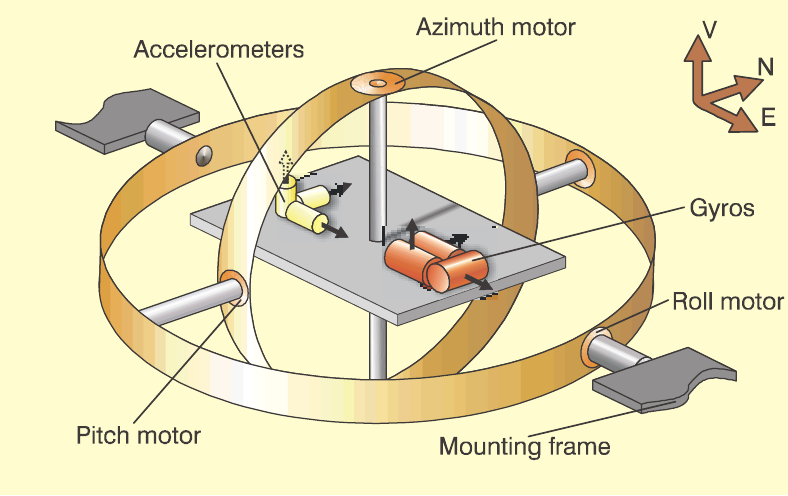
\includegraphics[scale=0.55]{images/gimbal.png} \cite{King98}
\end{frame}

\begin{frame}
	Vollkardanisch kreiselstabilisierte (Stabile Plattform)

	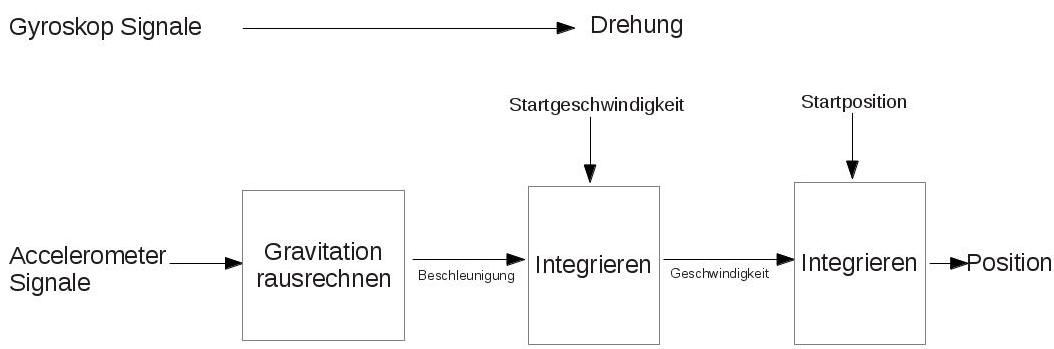
\includegraphics[width=\textwidth, height=0.4\textheight,keepaspectratio=true]{images/stable.jpg} 

	\bigskip
	Fahrzeugfeste (Strapdown)

		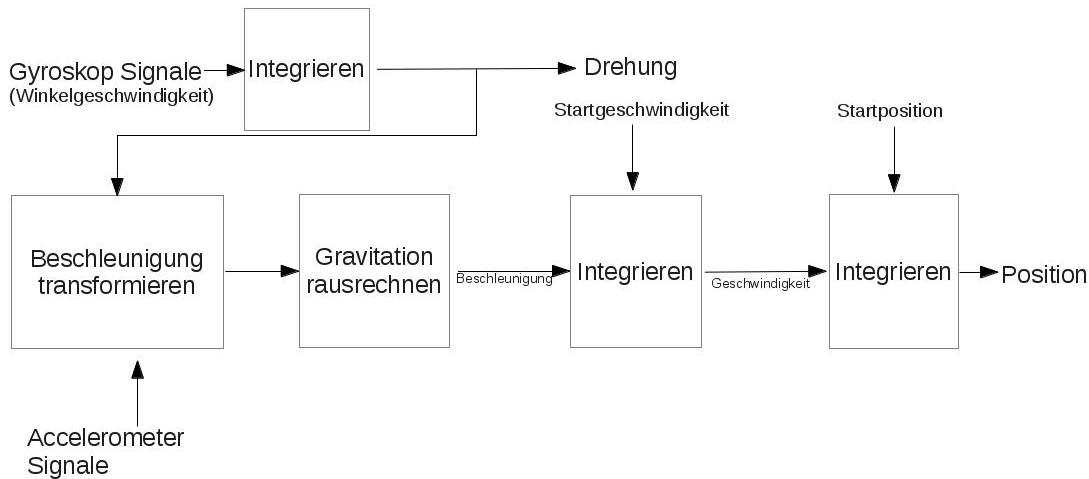
\includegraphics[width=\textwidth, height=0.4\textheight,keepaspectratio=true]{images/strap.jpg} 


\end{frame}

\begin{frame}
	\section{Autonome Flugkörper}
	\frametitle{Autonome Flugkörper}
	Bespiele: 
	
	\begin{itemize}
		\item Satelliten
		\item Raumfahrzeuge
		\item Flugzeuge mit Autopilot
		\item Marschflugkörper
	\end{itemize}
	
	Anforderungen an das INS:\\
	\begin{itemize}
		\item 20 Hz Update
		\item Mehre Stunden Flugzeit
		\item Kurzzeit Genauigkeit
	\end{itemize}
	
\end{frame}


\begin{frame}
  \section{Kalman-Filter}
  \frametitle{Kalman-Filter}
  \begin{itemize}
  	\item Problem:
  		\begin{itemize}
  			\item Abweichungen in den Sensordaten durch Aufsummierung von Fehlern, Rauschen im Prozess und in den Sensoren
  		\end{itemize}
  	\item Lösung:
  		\begin{itemize}
  			\item Vorausberechnung des nächsten Zustands des Systems mit Hilfe eines bekannten zu Grunde liegenden physikalischen Modells
  			\item Fusion aller zur Verfügung stehender Sensorwerte unabhängig von ihrer Genauigkeit Sensorwerte
  			\item gewichtetes Mittel dieser beiden Größen, um die Summe aller Fehlerquadrate zu minimieren
  		\end{itemize}
  \end{itemize}
  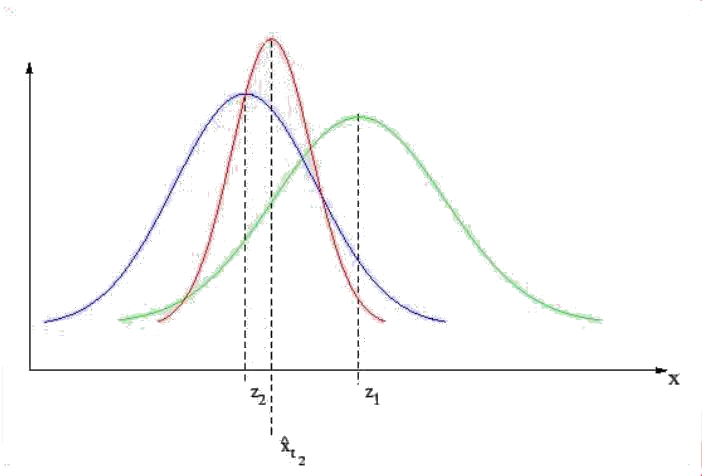
\includegraphics[width=0.4\textwidth]{images/Grundkurven.jpg}
\end{frame}

\begin{frame}
  \frametitle{Diskreter Kalman-Filter}
  \begin{itemize}
  	  \item einfacher Kalman-Filter
	  \item Swerling (1958), Kalman (1960), Kalman und Bucy (1961)
	  \item zuerst militärisch, heutzutage Anwendung in allen Bereichen der Mess- Steuer- und Regelungstechnik
  \end{itemize}
  \begin{definition}[Kalman-Filter]
  	Ein Kalman-Filter ist ein linearer, modellbasierender, stochastischer, rekursiver, gewichteter Schätz-Algorithmus zur Minimierung von Fehlerquadraten unbestimmer Messgrößen
  \end{definition}
  \begin{figure}[htbp]
        \begin{minipage}{0.3\textwidth}
         \centering
          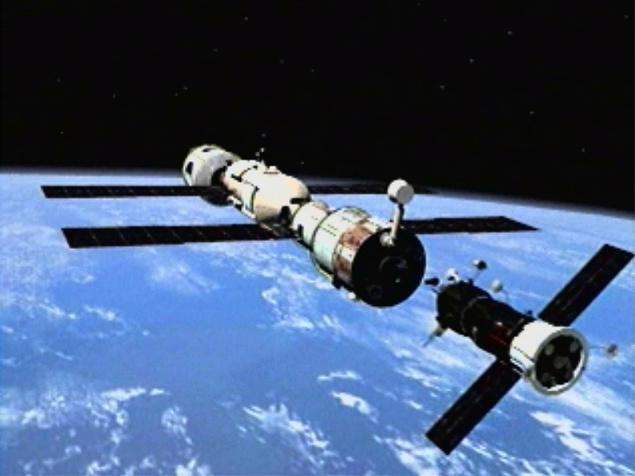
\includegraphics[width=0.8\textwidth]{images/docking.jpg}
          \caption{Präzisionsnavigation}
        \end{minipage}\hfill
        \begin{minipage}{0.3\textwidth}
         \centering
          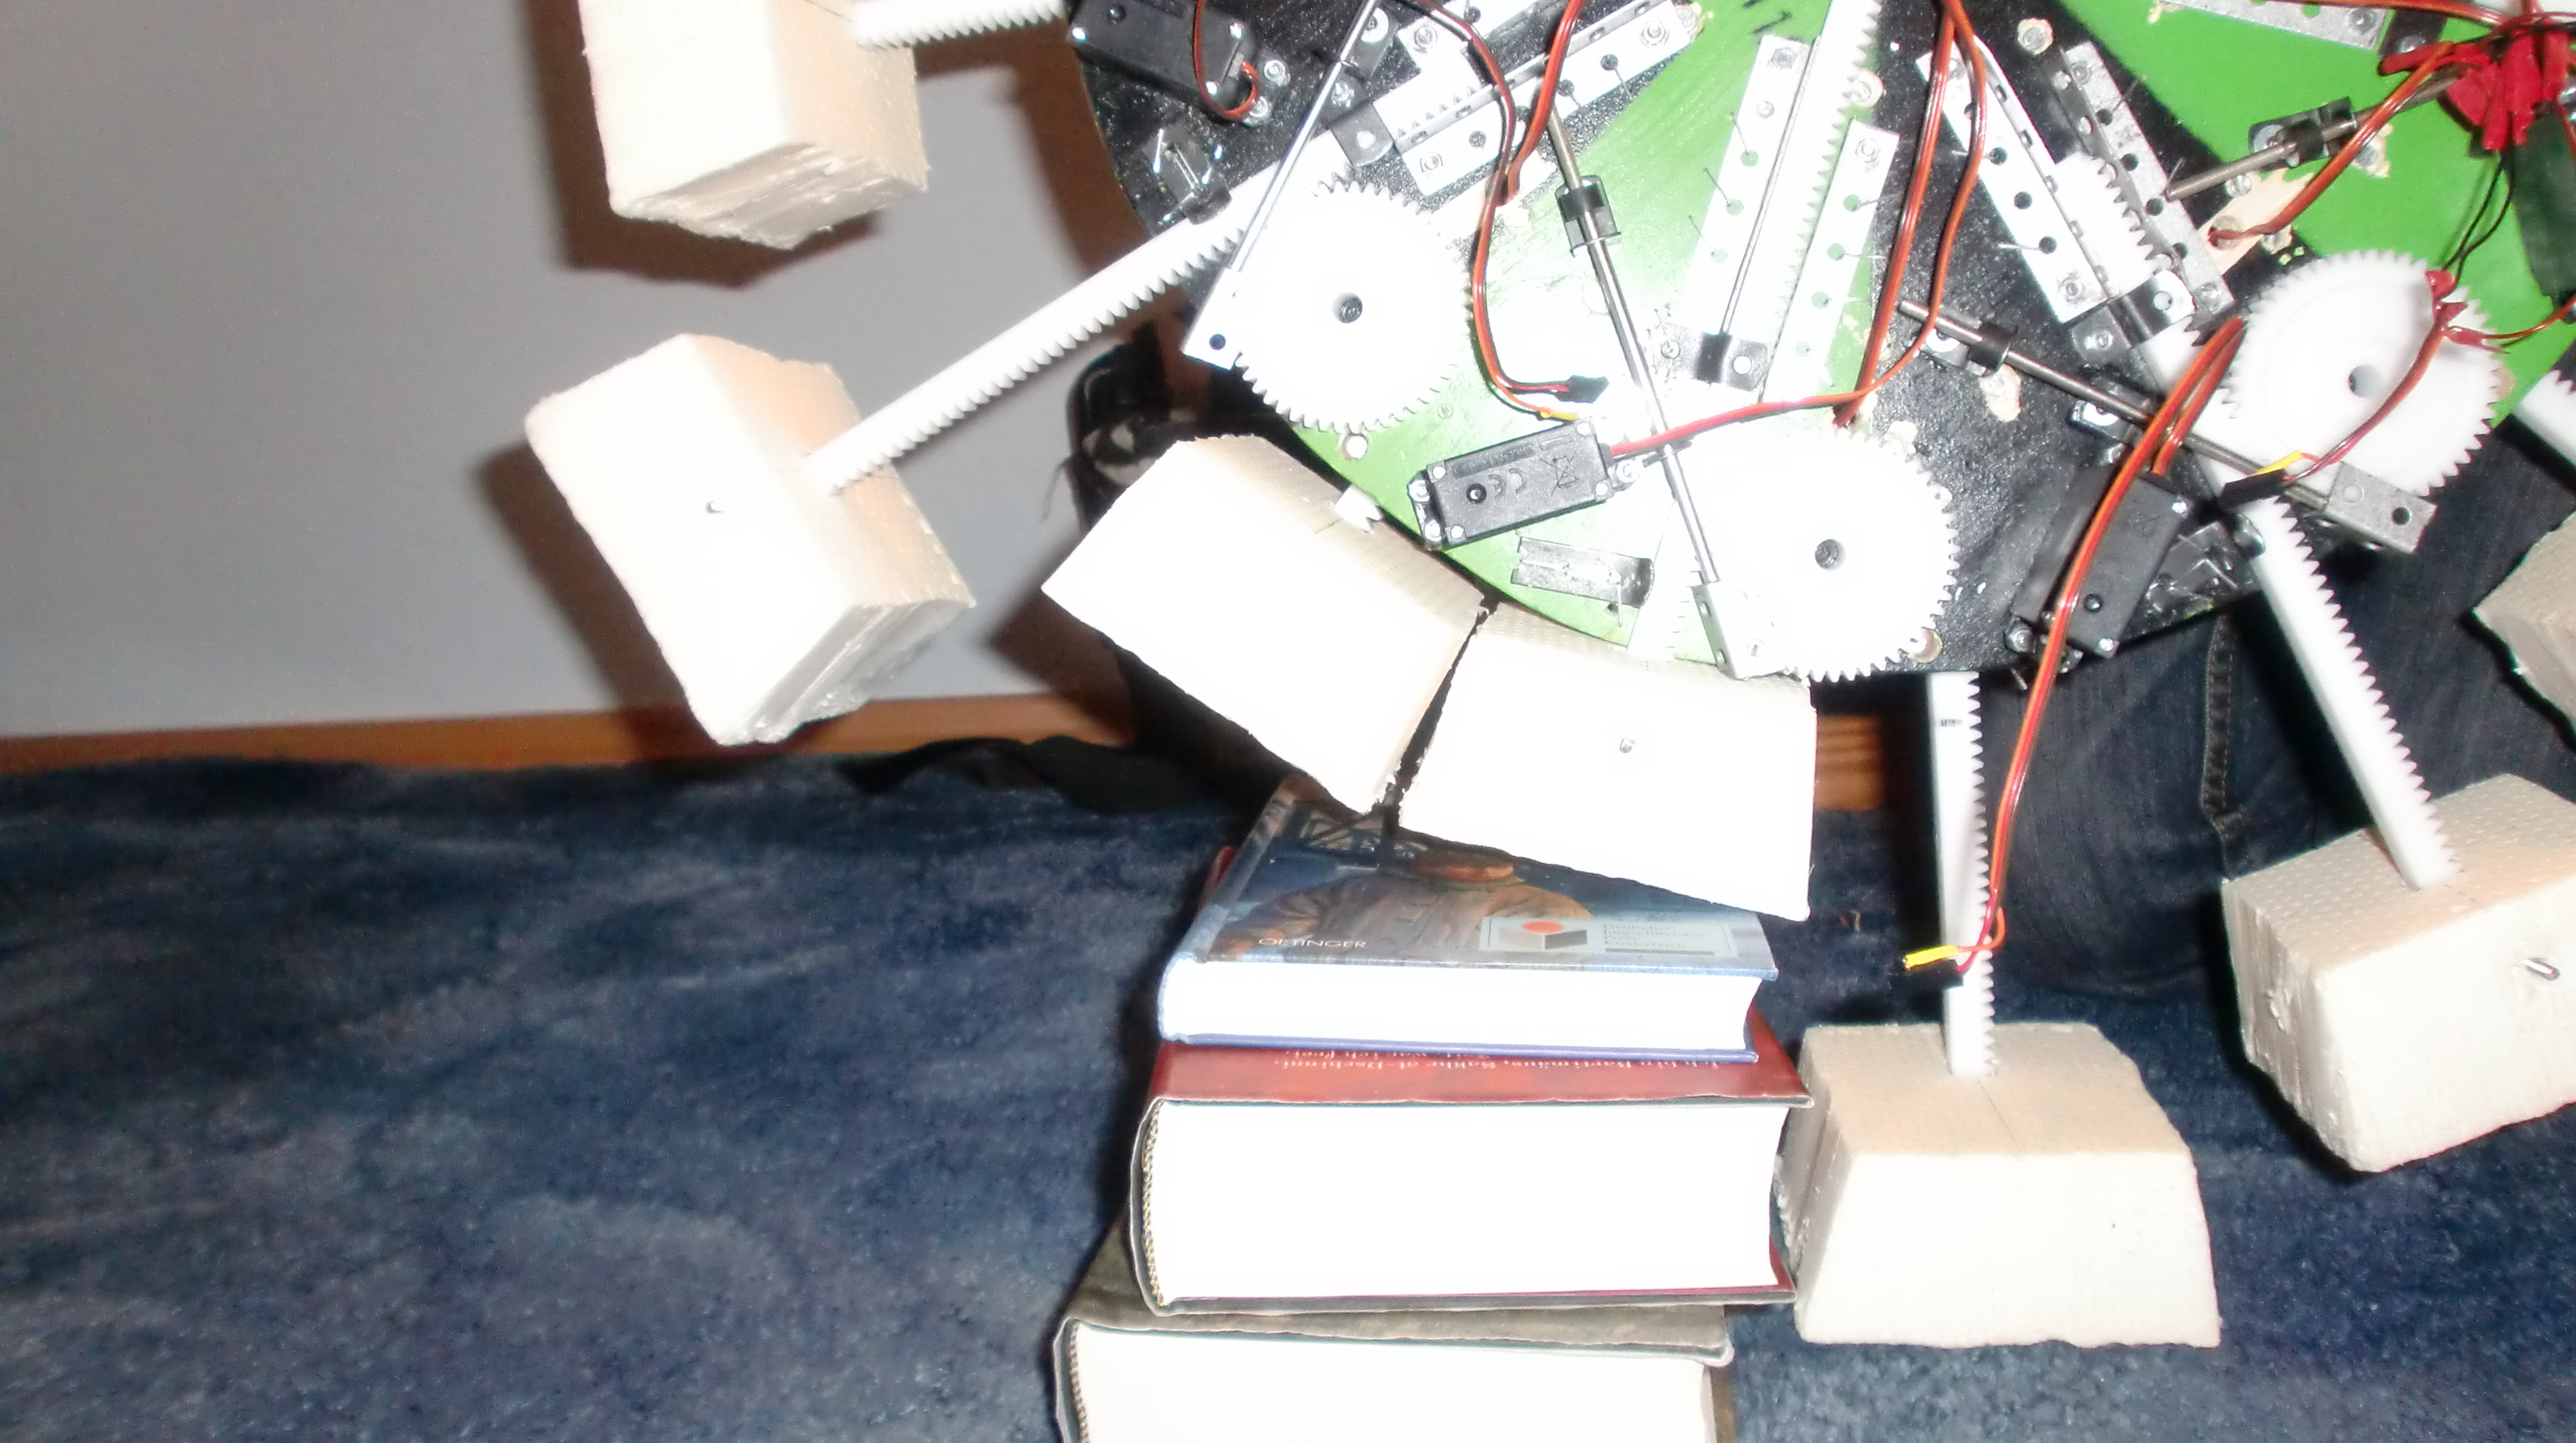
\includegraphics[width=0.8\textwidth]{images/smartwheel.jpg}
          \caption{Autonome technische Geräte jeder Art}
        \end{minipage}\hfill
        \begin{minipage}{0.3\textwidth}
         \centering
          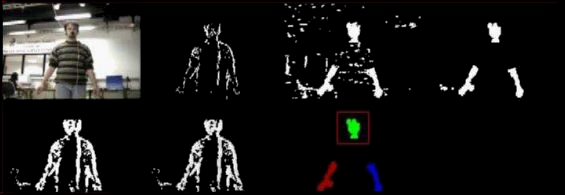
\includegraphics[width=0.8\textwidth]{images/head-tracking.jpg}
          \caption{Tracking von Körperteilen}
        \end{minipage}
      \end{figure}
\end{frame}
\begin{frame}
  \frametitle{Funktionsweise}
   \begin{figure}[htbp]
          \begin{minipage}{0.4\textwidth}
           \centering
            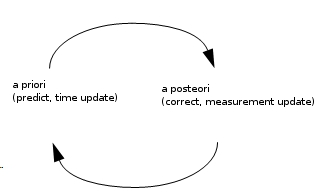
\includegraphics[width=0.8\textwidth]{images/grundfunktion.jpg}
          \end{minipage}\hfill
          \begin{minipage}{0.4\textwidth}
           \centering
            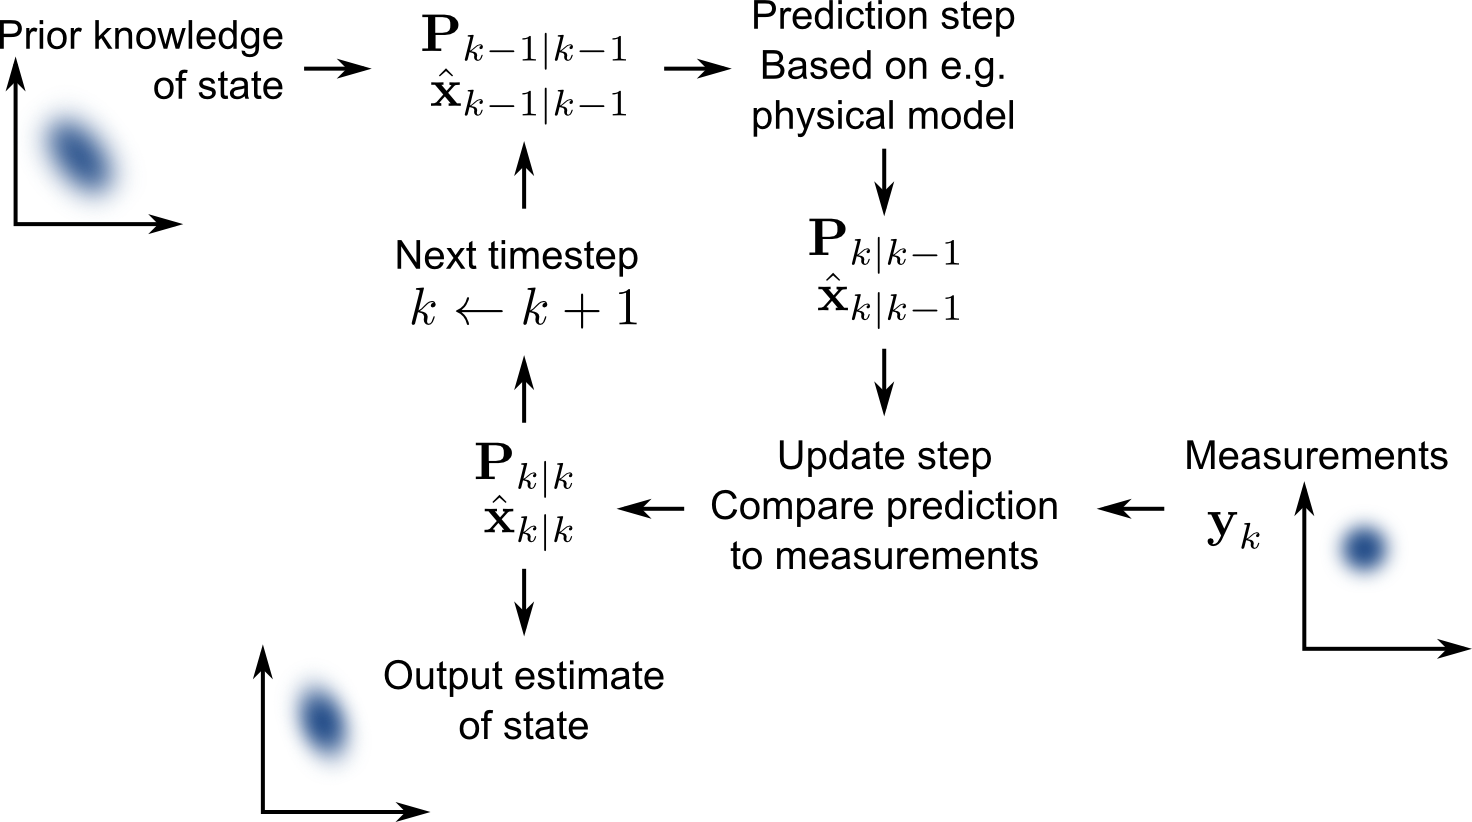
\includegraphics[width=0.8\textwidth]{images/Funktionsprinzip.png}
          \end{minipage}\hfill
   \end{figure}
\end{frame}

\begin{frame}
  \section{Literatur}
  \frametitle{Literatur}
\printbibliography

\end{frame}


\end{document}
